\chapter{مدل‌سازی و کنترل تک ربات‌}\label{ch one robot}
\section{مقدمه}
در این فصل چگونگی کنترل موقعیت برای هر یک از ربات‌ها توضیح داده شده است. در این پروژه از ربات‌های چرخدار دیفرانسیلی \LTRfootnote{Differential wheeled robot} استفاده شده است که ابتدا باید مدل ربات را به دست آورد. در این پروژه از مدل سینماتیکی \LTRfootnote{Kinematic model} ربات استفاده شده و وارد مدل دینامیکی نشده‌ایم. پس از توضیح مدل سینماتیکی، بر روی آن کنترل موقعیت پیاده سازی می‌شود. با توجه به مدلی که به دست آمده، می‌توان دریافت که متغیرهای کنترلی، سرعت چرخ های چپ و راست هستند و با کنترل آن‌ها و ادغام آن با سینماتیک معکوس، می‌توان کنترل موقعیت را انجام داد.

کنترل تک ربات دارای اهمیت بسیار زیادی است زیرا درون حلقه کنترل اجماع قرار می‌گیرد. حلقه داخلی باید 5 تا 10 برابر سریع‌تر از حلقه خارجی باشد تا کنترل کننده خارجی دچار مشکل نشود، در نتیجه سرعت پاسخ این کنترل کننده برای هدف نهایی بسیار اهمیت دارد.

حال که از اهمیت بالای این فصل آگاه شدیم، به بررسی نحوه بدست آوردن مدل سینماتیکی ربات‌ها می‌پردازیم.
 
\section{مدل‌سازی سینماتیکی}

در شکل \ref{Fig differential-robot} عکسی از ربات چرخدار دیفرانسیلی مشاهده می‌کنیم. 
\begin{figure}[!h]
	\centering
	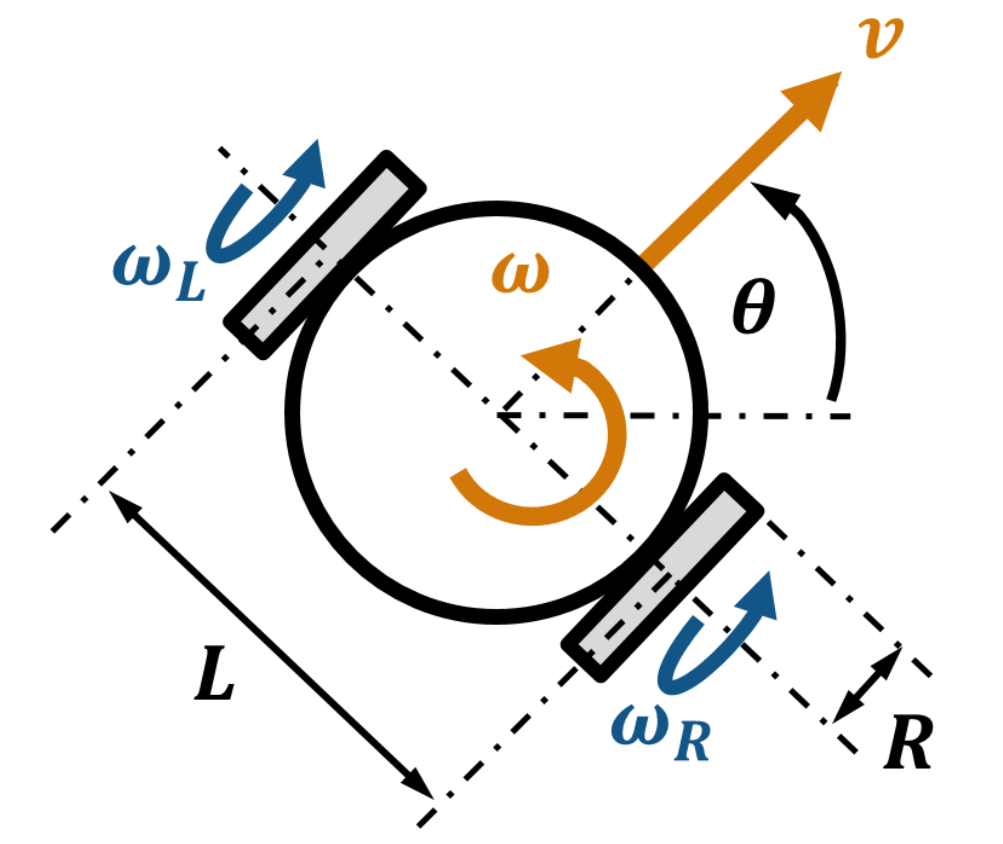
\includegraphics[scale=0.4]{Images/differential-robot-matlab.png}
	\caption{ربات استفاده شده به همراه پارامترهای آن}\label{Fig differential-robot}
\end{figure}

ورودی این ربات $\omega_L$ و $\omega_R$ که سرعت زاویه ای چرخ چپ و راست است، می‌باشد. همچنین خروجی ربات، سرعت خطی ربات، 
\verb|v|، و سرعت زاویه ای ربات، $\omega$ است. شعاع چرخ، 
\verb|R|، و فاصله بین دو چرخ، 
\verb|L|، مشخصات فیزیکی ربات هستند. در نهایت موقعیت ربات توسط مکان مرکز آن در بیان صفحه مختصات 
\verb|y|-\verb|x| و همچنین اختلاف زاویه رو به روی ربات با محور 
 \verb|x|  ها، با $\theta$ بیان می‌شود.

با توجه به شکل \ref{Fig circle-arc} اگر زاویه قطاع را $\theta$ بگیریم، داریم:
\begin{equation}
s = r\theta
\end{equation}

\begin{figure}[!h] 
	\centering
	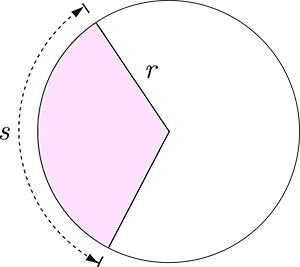
\includegraphics[scale=2]{Images/Circle_arc2.jpg}
	\caption{دایره به همراه قطاع و کمان آن} \label{Fig circle-arc}
\end{figure}

پس اگر چرح را کاملا دایره فرض کنیم و طول کمان را همچنان \verb|s| بگیریم، خواهیم داشت:
\begin{equation}
s = R\theta
\end{equation}

سپس با صرف نظر از تغییرات شعاع چرخ، به کمک یک مشتق به رابطه بین سرعت خطی و سرعت زاویه ای برای هر چرخ می‌رسیم:
\begin{equation} \label{eq wheel v w}
v = \dot{s} = R\dot{\theta} = R\omega
\end{equation}

سرعت خطی ربات با میانگین سرعت خطی هر چرخ برابر است. پس لگر سرعت خطی چرخ راست و چپ را به ترتیب با $v_{R}$ و $v_{L}$ نشان دهیم، داریم:
\begin{equation} \label{eq linear velocity}
v = \frac{v_R + v_L}{2}
\end{equation}

با ادغام روابط \ref{eq wheel v w} و \ref{eq linear velocity} داریم:
\begin{equation} \label{eq forward kinematics v}
v = \frac{R}{2}(\omega_R + \omega_L)
\end{equation}

برای محاسبه سرعت زاویه ای ربات از \verb|ICC| \LTRfootnote{Instantaneous center of curvature} استفاده می‌شود که ربات همانند شکل \ref{Fig differential-robot-ICC} حول آن دوران می‌کند. قابل توجه است که چون دو چرخ آخر خودرو آزادی عمل ندارند، می توان خودرو را با ربات چرخدار دیفرانسیلی مدل کرد.
\begin{figure}[!h] 
	\centering
	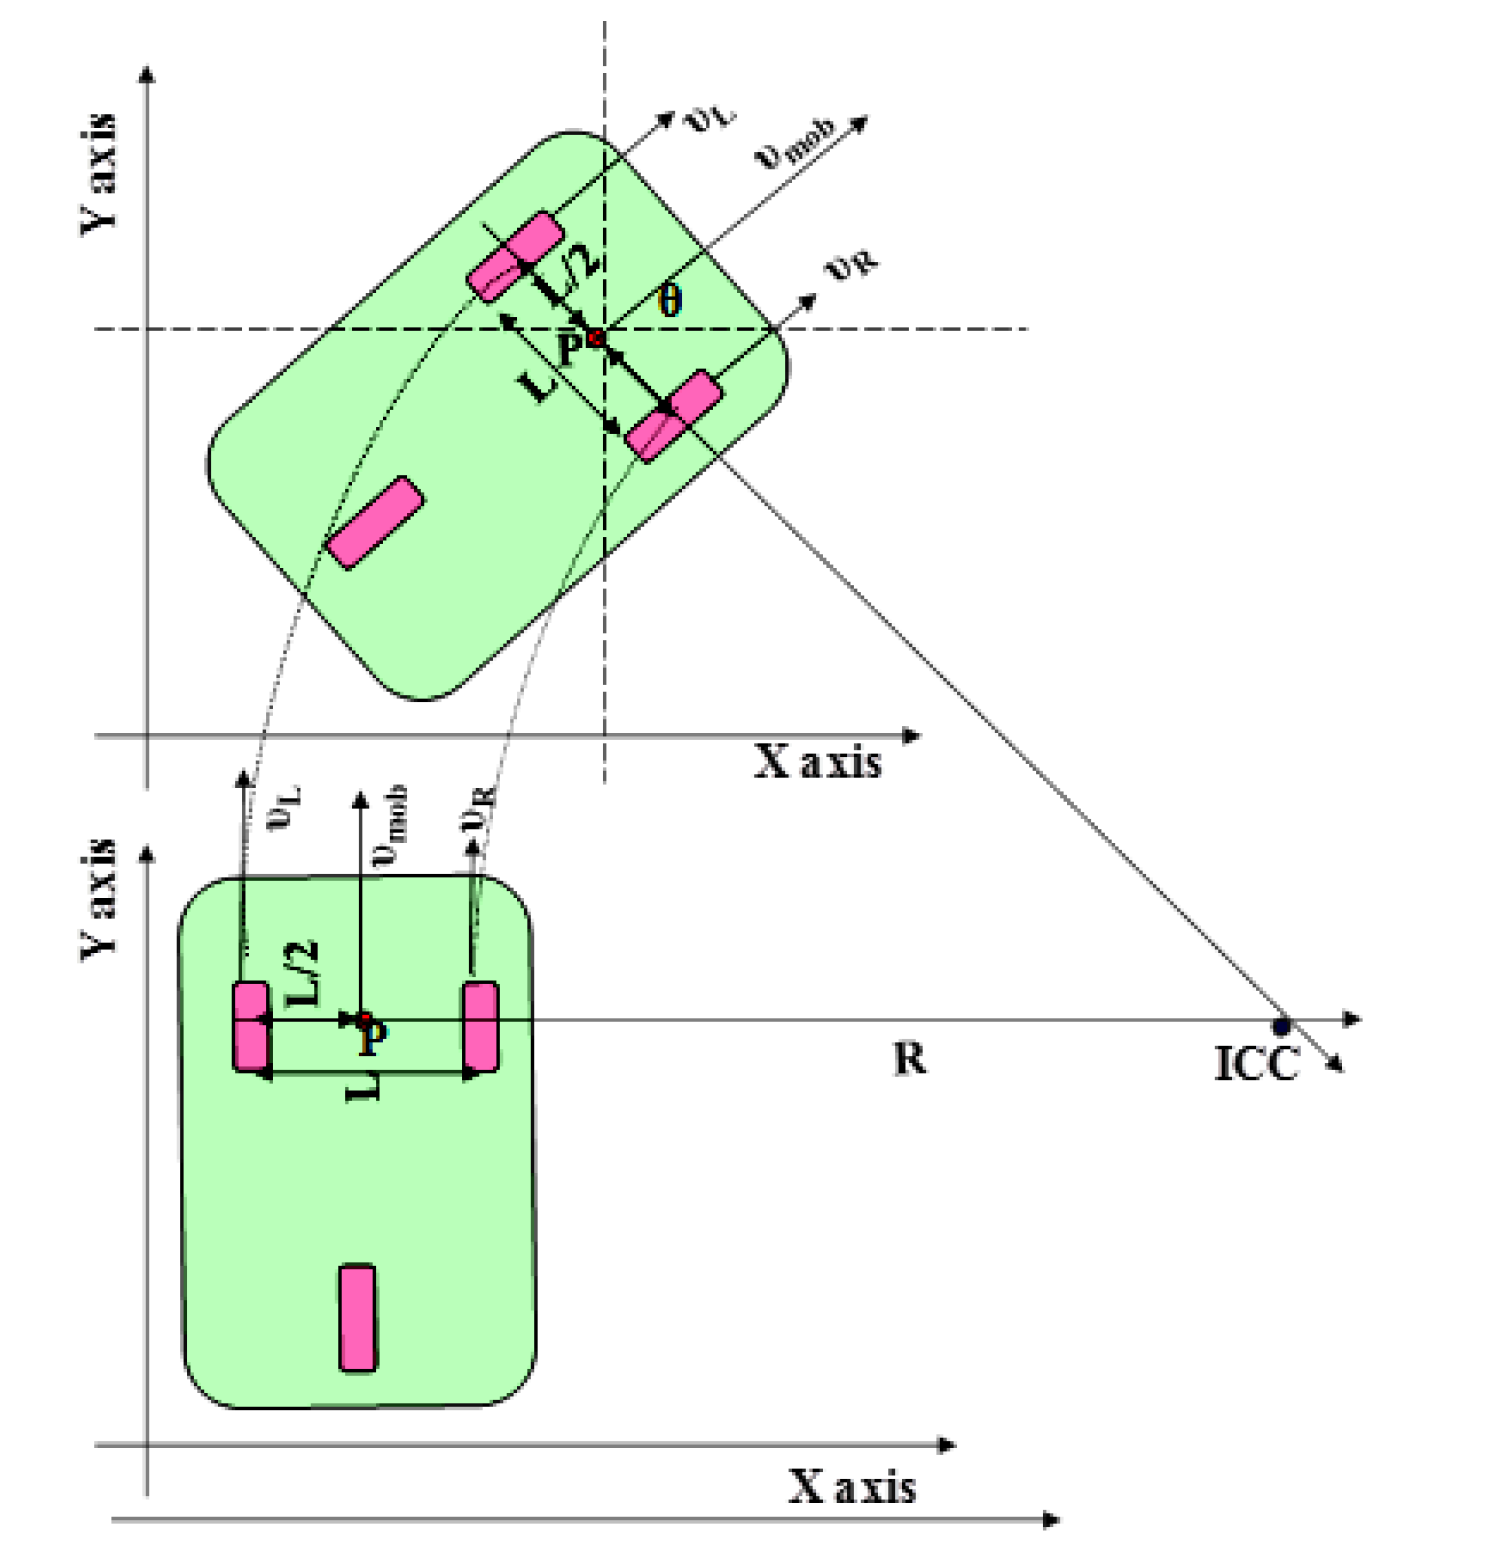
\includegraphics[scale=0.28]{Images/differential-robot-ICC.png}
	\caption{چرخش ماشین حول یک نقطه مشخص} \label{Fig differential-robot-ICC}
\end{figure}

مقدار \verb|ICC| طبق رابطه زیر به دست می‌آید:
\begin{equation}
ICC = (x - Rsin(\theta), y + Rcos(\theta))
\end{equation}
 که \verb|R| فاصله بین مرکز دو چرخ جلوی خودرو و نقطه‌ای است که حول آن دوران می‌کند. پس داریم:
 
\begin{equation} \label{eq ICC radius}
R = \frac{L}{2} \times \frac{v_L + v_R}{v_L - v_R}
\end{equation}

حال اگر دایره را به مرکز \verb|ICC| و شعاع \verb|R| در نظر بگیریم، با توجه به روابط \ref{eq wheel v w}، \ref{eq linear velocity} و \ref{eq ICC radius} داریم:
\begin{equation} \label{eq forward kinematics w}
\omega = \frac{v}{R} = \frac{R}{L}(v_R - v_L)
\end{equation}

در نتیجه با توجه به معادلات \ref{eq forward kinematics v} و \ref{eq forward kinematics w}، سینماتیک معکوس ربات برابر است با:
\begin{equation} \label{eq inverse kinematics}
\omega_L = \frac{1}{R}(v - \frac{\omega L}{2}),~~~  \omega_R = \frac{1}{R}(v + \frac{\omega L}{2})
\end{equation}

حال اگر در کنترل کننده موقعیت، مقدار \verb|v| و $\omega$ را محاسبه کرد، می‌توان به کمک رابطه \ref{eq inverse kinematics} سرعت زاویه‌ای چرخ‌ها را طوری تنظیم نمود که ربات به سرعت خطی و زاویه‌ای ایده‌آل خود برسد.

\section{کنترل کننده موقعیت تک ربات}

در این قسمت هدف این است که موقعیت ربات، یا به عبارتی مختصات مرکز ربات را در صفحه \verb|y|-\verb|x| کنترل کرد. متغیر کنترلی، سرعت زاویه‌ای چرخ‌ها می باشد. حال هدف این است که با محاسبه خطا و به کمک کنترل کننده، خروجی کنترل کننده را به سرعت خطی و زاویه‌ای ربات تبدیل کنیم تا در نهایت با کمک از رابطه سینماتیک معکوس \ref{eq inverse kinematics} بتوان به سرعت زاویه‌ای چرخ‌ها رسید.

\subsection{کنترل سرعت زاویه‌ای ربات}
در این کنترل ‌کننده هدف ما این است که سر ربات به سمت موقعیت مرجع باشد. در نتیجه پس از محاسبه خطا داریم:
\begin{equation}
e = 
\begin{bmatrix}
x_d - x \\
y_d - y
\end{bmatrix}
\end{equation}

که در آن $x_d$ و $y_d$ موقعیت مرجع و \verb|x| و \verb|y| موقعیت فعلی ربات هستند.

حال با توجه به خطای به دست آمده، با کمک از تابع \verb|Atan2| زاویه‌ای که ربات باید در آن جهت قرار بگیرد، محاسبه می‌گردد. مزیت استفاده از این تابع این است که برد آن در بازه
$-\pi$
تا
$\pi$
می‌باشد و باعث می‌شود که جهت رو‌به‌روی ربات اهمیت پیدا کند. قابل ذکر است که اگر از \verb|arctan| استفاده می‌شد، آنگاه فقط راستای رو‌به‌روی ربات اهمیت پیدا می‌کرد و برای حالتی که ربات رو به نقطه مرجع یا پشت به آن می‌باشد، فرقی قائل نمی‌شد.

در شکل \ref{Fig atan2} دامنه و برد تابع \verb|Atan2| قابل مشاهده است.
\begin{figure}[!h] 
	\centering
	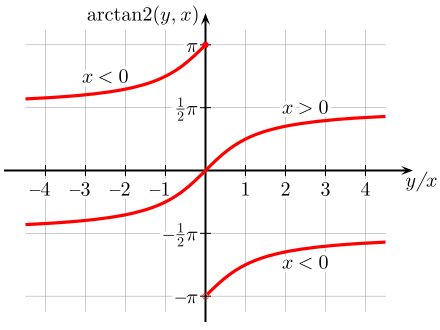
\includegraphics[scale=0.8]{Images/atan2.png}
	\caption{دامنه و برد تابع استفاده شده} \label{Fig atan2}
\end{figure}

اکنون با کمک این تابع زاویه‌ای که ربات باید در آن جهت قرار گیرد، $\theta_d$، به صورت زیر محاسبه می‌گردد:
\begin{equation}
\theta_d = Atan2(y_d - y, x_d - x)
\end{equation}
که ورودی‌های تابع، عناصر بردار خطا هستند.

حال که زاویه مرجع به دست آمد، با کم کردن زاویه حال حاضر ربات، به خطای زاویه می‌رسیم. سپس با استفاده از کنترل کننده انتگرال‌گیر نسبت، به سرعت زاویه‌ای ربات دست پیدا می‌کنیم. در نتیجه با تنظیم سرعت زاویه‌ای چرخ‌ها به طوری که به سرعت زاویه‌ای مد نظر در ربات برسیم، می‌توان چهت‌گیری ربات را کنترل نمود. در قسمت بعد، به چگونگی کنترل سرعت خطی ربات پرداخته خواهد شد. 

\subsection{کنترل سرعت خطی ربات}
برای کنترل سرعت خطی ربات، فاصله بین مکان حال تا موفعیت هدف، به عنوان ورودی کنترلی مد نظر قرار می‌گیرد. قابل ذکر است که این فاصله برابر با نرم دو بردار اختلاف این دو موقعیت است و از این رابطه در کنترل استفاده شده است. در نتیجه ورودی کنترلی برابر است با:
\begin{equation}
\|e\|_2 = \sqrt{(x_d - x)^{2} + (y_d - y)^{2}}
\end{equation}

در این قسمت از کنترل کننده نسبت مشتق‌گیر\LTRfootnote{PD} استفاده شده است. دلیل استفاده نیز این بود که سرعت ربات دارای اهمیت است، در نتیجه از انتگرال‌گیر که سرعت را کاهش می‌دهد، استفاده نشده است. ار طرفی چون پاسخ گذرا هنگام کنترل سرعت دارای اهمیت است، از مشتق‌گیر استفاده شده است تا پاسخ را بهبود بخشد. همچنین برای جلوگیری از وارد شدن ولتاژ بیش از حد به ربات، در خروجی کنترلی اشباع قرار داده شده است تا سرعتی که از ربات می خواهیم و در نتیجه ولتاژ اعمالی به موتور چرخ ها، محدود گردد.

حال نتایج آزمایشات برای یک ربات، مورد بررسی قرار می‌گیرد.

\section{نتایج کنترل موقعیت یک ربات}

 
\index{کتاب}
\index{پارسی‌لاتک}
\index{بی‌دی}
\index{سوال}
\index{عنصر}
\index{گزینه}
\index{ژاکت}
\index{مرکز دانلود}
\index{اجرا}
\index{تک‌لایو}
\index{ثالث}
\index{جهان}
\index{چهار}
\index{حمایت}
\index{خواهش}
\index{دنیا}
\index{زی‌پرشین}
\index{ریحان}
\index{شیرین}
\index{صمیمی}
\index{ضمیر}
\index{طبیب}